\chapter{La mécanique quantique du chimiste~: systèmes modèles}\label{ch:b3:quantum-model-systems}

Trois petites fioles sont posées sur la paillasse, chacune contenant une
solution d'un colorant cyanine dans l'éthanol~: la première est magenta,
la deuxième bleue, la troisième d'un bleu verdâtre profond qui absorbe
dans le rouge lointain. Les trois molécules sont bâties sur le même
modèle --- deux cycles azotés identiques reliés par une chaîne d'atomes de
carbone --- et ne diffèrent que par la longueur de cette chaîne, de deux
atomes de carbone en deux. Allonger la chaîne déplace la couleur vers le
rouge. En 1949, un chimiste a expliqué cette série par l'un des problèmes
les plus simples de la mécanique quantique~: un électron libre de se
déplacer sur un segment de longueur fixe, une «~\omterm{def:b3:quantum-model-systems:box}{particule dans une
boîte}~». Ce chapitre met en place l'outillage qui sous-tend cette
explication --- \omterm{def:b3:quantum-model-systems:operator}{opérateurs}, \omterm{def:b3:quantum-model-systems:operator}{valeurs propres}, \omterm{thm:b3:quantum-model-systems:schrodinger}{équation de Schrödinger} ---
et résout les systèmes modèles dont la chimie se sert tous les jours~: la
boîte, l'\omterm{def:b3:quantum-model-systems:oscillator}{oscillateur harmonique} d'une liaison qui vibre, le \omterm{def:b3:quantum-model-systems:rotor}{rotateur
rigide} d'une molécule qui tourne, l'atome d'hydrogène, et la barrière
qu'une particule légère peut franchir sans avoir l'énergie de la gravir.

\begin{recall}
Le volume de première année a montré que l'énergie d'un atome est
quantifiée (niveaux d'énergie, état fondamental et états excités, raies
de l'hydrogène) et qu'un photon transporte $E = h\nu = hc/\lambda$. Le
volume de deuxième année a décrit un électron par une fonction d'onde
$\psi$ dont le carré est une densité de probabilité, a séparé les
orbitales de l'hydrogène en parties radiale et angulaire et a compté
leurs nœuds~; il a pris les fonctions d'onde de l'hydrogène comme
données. Elles sont établies ici, à la section 5. De la physique~: la
quantité de mouvement $p = mv$ et la longueur d'onde de de Broglie
$\lambda = h/p$.
\end{recall}

\begin{omfigure}
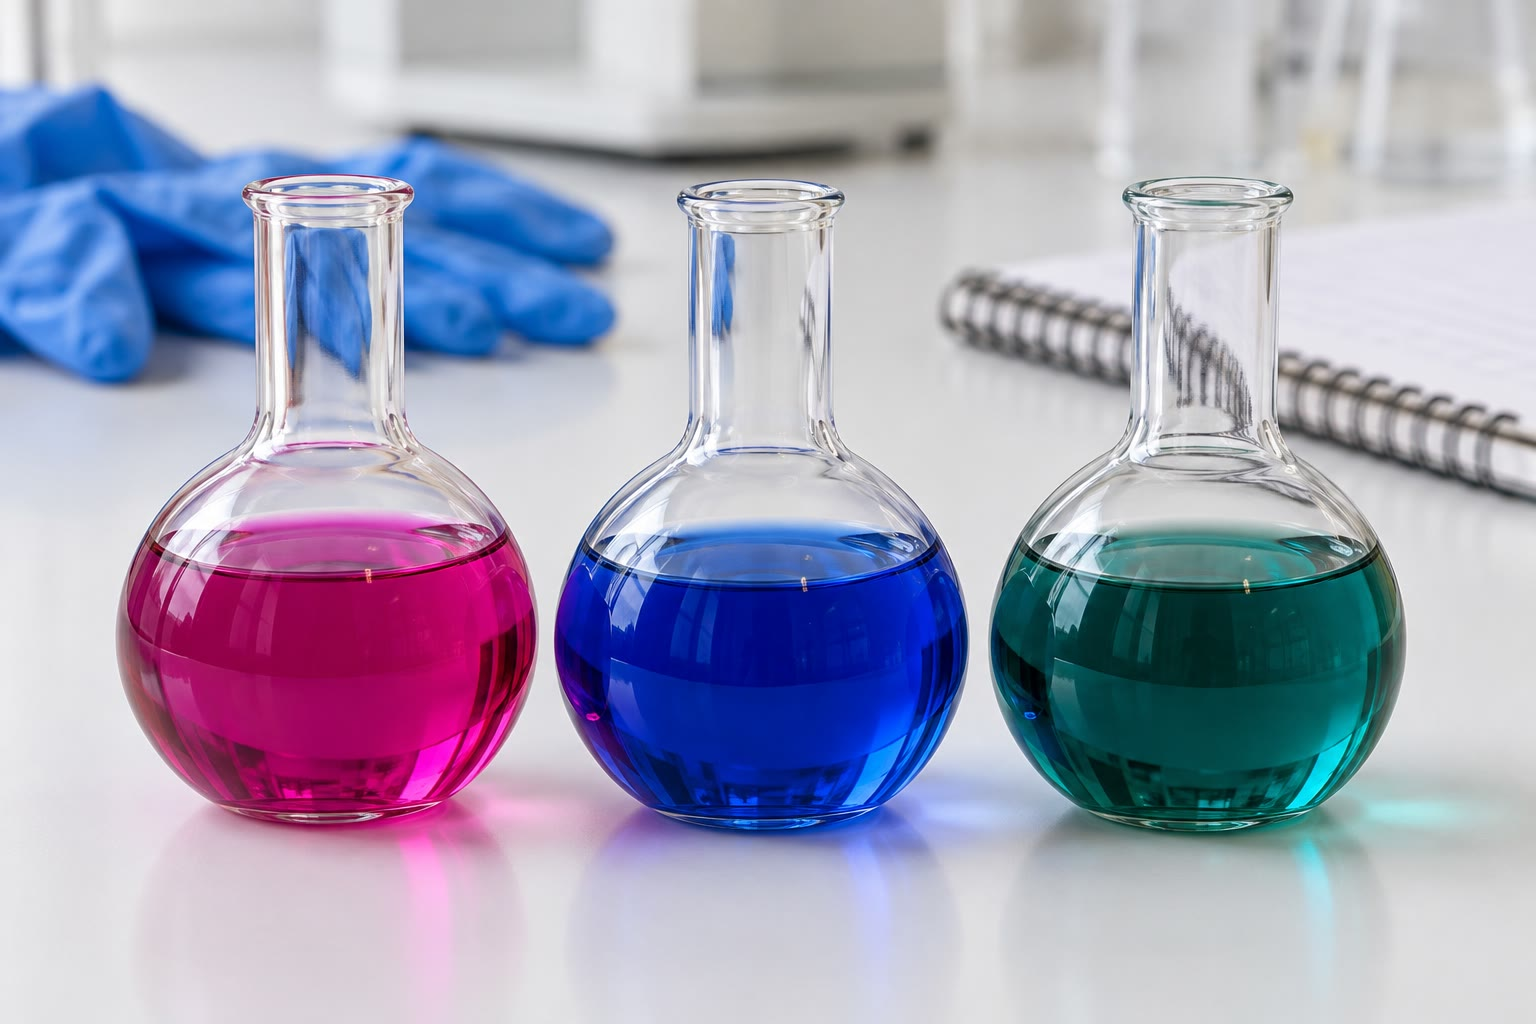
\includegraphics[width=0.62\linewidth]{images/book4/ai/b3-01-dyes.jpg}

{\small Solutions de trois colorants cyanines d'une même famille. Chaque
paire d'atomes de carbone ajoutée à la chaîne déplace l'absorption vers
le rouge.}
\end{omfigure}

\section{Opérateurs, valeurs propres et équation de Schrödinger}

La mécanique classique attribue à une particule une position et une
quantité de mouvement à chaque instant. La mécanique quantique lui
attribue un état, la fonction d'onde $\psi$, et remplace chaque grandeur
mesurable par une opération effectuée sur $\psi$.

\begin{definition}[Opérateur, fonction propre, valeur propre]\label{def:b3:quantum-model-systems:operator}
Un \emph{opérateur}\index{operateur@opérateur} $\hat A$ est une règle qui
transforme une fonction en une autre fonction~: $\hat A f = g$. Il est
linéaire si $\hat A(\lambda f +
\mu g) = \lambda\hat Af + \mu\hat Ag$. Une fonction non nulle $f$ telle que
$\hat Af = a f$ pour un nombre $a$ est une \emph{fonction propre}\index{fonction propre}
de $\hat A$, et $a$ est la \emph{valeur propre}\index{valeur propre} associée.
\end{definition}

\begin{example}[Deux opérateurs~: position et quantité de mouvement]\label{ex:b3:quantum-model-systems:xp}
À une dimension, l'\omterm{def:b3:quantum-model-systems:operator}{opérateur} position multiplie par $x$, $\hat x f = xf$,
et l'\omterm{def:b3:quantum-model-systems:operator}{opérateur} quantité de mouvement dérive, $\hat p f = -\iu\hbar\,
\dd f/\dd x$, avec $\hbar = h/2\pi$. La fonction $\eu^{\iu kx}$ est une
\omterm{def:b3:quantum-model-systems:operator}{fonction propre} de $\hat p$ de \omterm{def:b3:quantum-model-systems:operator}{valeur propre} $\hbar k$~: une onde de
longueur d'onde $\lambda = 2\pi/k$ a une quantité de mouvement
$h/\lambda$, c'est la relation de de Broglie. La fonction $\sin kx$ n'est
pas \omterm{def:b3:quantum-model-systems:operator}{fonction propre} de $\hat p$ (sa dérivée est un cosinus), mais elle
l'est de $\hat p^2 = -\hbar^2\,\dd^2/\dd x^2$, avec la \omterm{def:b3:quantum-model-systems:operator}{valeur propre}
$\hbar^2k^2$.
\end{example}

\begin{definition}[Opérateur hermitien, valeur moyenne]\label{def:b3:quantum-model-systems:hermitian}
On note $\langle f|g\rangle = \int f^*g\,\dd\tau$ pour deux fonctions qui
s'annulent aux bords de la région. Un \omterm{def:b3:quantum-model-systems:operator}{opérateur} est dit
\emph{hermitien}\index{operateur hermitien@opérateur hermitien}
si $\langle f|\hat Ag\rangle = \langle \hat Af|g\rangle$ pour toutes ces
fonctions $f$ et $g$. Pour un état normé $\psi$ ($\langle\psi|\psi\rangle = 1$),
la \emph{valeur moyenne}\index{valeur moyenne} de $\hat A$ est
$\langle A\rangle = \langle\psi|\hat A\psi\rangle$~: la moyenne d'un grand
nombre de mesures faites sur des systèmes préparés à l'identique.
\end{definition}

Les règles de travail de la chimie quantique --- ses postulats --- se
disent maintenant d'une traite~: toute grandeur mesurable est représentée
par un \omterm{def:b3:quantum-model-systems:hermitian}{opérateur hermitien}~; une mesure donne l'une de ses \omterm{def:b3:quantum-model-systems:operator}{valeurs
propres}~; et si $\psi$ est \omterm{def:b3:quantum-model-systems:operator}{fonction propre} de $\hat A$, toute mesure
effectuée sur cet état donne la même valeur, sa \omterm{def:b3:quantum-model-systems:operator}{valeur propre}.

\begin{theorem}[Opérateurs hermitiens]\label{thm:b3:quantum-model-systems:hermitian-real}
Les \omterm{def:b3:quantum-model-systems:operator}{valeurs propres} d'un \omterm{def:b3:quantum-model-systems:hermitian}{opérateur hermitien} sont réelles. Deux \omterm{def:b3:quantum-model-systems:operator}{fonctions
propres} associées à des \omterm{def:b3:quantum-model-systems:operator}{valeurs propres} différentes sont orthogonales~:
$\langle f_1|f_2\rangle = 0$.
\end{theorem}

\begin{proof}
Soit $\hat Af = af$. Alors $\langle f|\hat Af\rangle = a\langle f|f\rangle$ et
$\langle\hat Af|f\rangle = a^*\langle f|f\rangle$. L'\omterm{def:b3:quantum-model-systems:operator}{opérateur} est
\omterm{def:b3:quantum-model-systems:hermitian}{hermitien}, donc les deux sont égaux, et $\langle f|f\rangle > 0$~: $a = a^*$.
Soient maintenant $\hat Af_1
= a_1f_1$ et $\hat Af_2 = a_2f_2$ avec $a_1 \ne a_2$, toutes deux réelles. Alors
$\langle f_1|\hat Af_2\rangle = a_2\langle f_1|f_2\rangle$ et $\langle\hat Af_1|
f_2\rangle = a_1\langle f_1|f_2\rangle$~; leur égalité donne $(a_2 - a_1)
\langle f_1|f_2\rangle = 0$, d'où $\langle f_1|f_2\rangle = 0$.
\end{proof}

Une valeur mesurée est un nombre réel, et c'est pourquoi les observables
doivent être hermitiennes~; l'orthogonalité est ce qui fait des orbitales
d'un atome, ou des niveaux d'une boîte, un ensemble propre d'états
indépendants.

\begin{definition}[Commutateur]\label{def:b3:quantum-model-systems:commutator}
Le \emph{commutateur}\index{commutateur} de deux \omterm{def:b3:quantum-model-systems:operator}{opérateurs} est $[\hat A,\hat B] =
\hat A\hat B - \hat B\hat A$. Les \omterm{def:b3:quantum-model-systems:operator}{opérateurs} commutent si leur commutateur
est nul.
\end{definition}

\begin{example}[Le commutateur canonique]\label{ex:b3:quantum-model-systems:canonical}
Pour toute fonction $f$, $\hat x\hat pf = -\iu\hbar xf'$ et $\hat p\hat xf =
-\iu\hbar(f + xf')$. La différence vaut $[\hat x,\hat p]f = \iu\hbar f$, donc
$[\hat x,\hat p] = \iu\hbar$~: la position et la quantité de mouvement ne
commutent pas. Cette seule relation fonde le principe d'incertitude et,
plus loin, tout le spectre de l'\omterm{def:b3:quantum-model-systems:oscillator}{oscillateur harmonique}.
\end{example}

\begin{proposition}[Opérateurs qui commutent]\label{prop:b3:quantum-model-systems:commuting}
Si $\hat A$ et $\hat B$ commutent et si $f$ est \omterm{def:b3:quantum-model-systems:operator}{fonction propre} de $\hat A$
associée à une \omterm{def:b3:quantum-model-systems:operator}{valeur propre} non dégénérée $a$, alors $f$ est aussi
\omterm{def:b3:quantum-model-systems:operator}{fonction propre} de $\hat B$.
\end{proposition}

\begin{proof}
$\hat A(\hat Bf) = \hat B\hat Af = a(\hat Bf)$~: la fonction $\hat Bf$ est
\omterm{def:b3:quantum-model-systems:operator}{fonction propre} de $\hat A$ avec la même \omterm{def:b3:quantum-model-systems:operator}{valeur propre} $a$, ou bien nulle.
La \omterm{def:b3:quantum-model-systems:operator}{valeur propre} étant non dégénérée, $\hat Bf$ est un multiple de $f$,
disons $bf$.
\end{proof}

L'\omterm{def:b3:quantum-model-systems:operator}{opérateur} associé à l'énergie est le hamiltonien. Pour une particule de
masse $m$ dans un potentiel $V$, l'énergie classique $p^2/2m + V$ devient
un \omterm{def:b3:quantum-model-systems:operator}{opérateur}.

\begin{definition}[Opérateur hamiltonien]\label{def:b3:quantum-model-systems:schrodinger}
L'\emph{opérateur hamiltonien}\index{operateur hamiltonien@opérateur hamiltonien} d'une particule de
masse $m$ qui se déplace dans un potentiel $V(\mathbf r)$ est
\[
\hat H = -\frac{\hbar^2}{2m}\nabla^2 + V(\mathbf r), \qquad \nabla^2 =
\frac{\partial^2}{\partial x^2} + \frac{\partial^2}{\partial y^2} +
\frac{\partial^2}{\partial z^2},
\]
et, pour plusieurs particules, la somme de leurs termes cinétiques et de
toutes leurs énergies potentielles.
\end{definition}

\begin{theorem}[L'équation de Schrödinger]\label{thm:b3:quantum-model-systems:schrodinger}
Les états d'énergie bien définie d'un système --- ses états
stationnaires --- sont les \omterm{def:b3:quantum-model-systems:operator}{fonctions propres} de son hamiltonien, et ses
énergies permises sont les \omterm{def:b3:quantum-model-systems:operator}{valeurs propres}~:
\[
\hat H\psi = E\psi,
\]
l'\emph{équation de Schrödinger}\index{equation de Schrodinger@équation de Schrödinger} indépendante du temps.
Une fonction $\psi$ acceptable est univoque, continue et de carré
sommable (elle peut être normée).
\end{theorem}
\begin{proof}[Statut]
C'est un postulat, justifié par ses conséquences~: les niveaux de tous
les systèmes résolus ci-dessous s'accordent avec la spectroscopie.
L'équation dépendant du temps, dont celle-ci est le cas stationnaire,
relève de la physique.
\end{proof}

Ce sont les conditions aux limites qui quantifient~: une équation
différentielle a des solutions pour toute valeur de $E$, mais seul un
ensemble discret d'entre elles reste fini et continu. La chimie consiste
alors à choisir un potentiel, à résoudre et à lire les \omterm{def:b3:quantum-model-systems:operator}{valeurs propres}.

\begin{method}[Résoudre un modèle à une dimension]\label{met:b3:quantum-model-systems:one-dimensional}
\begin{enumerate}
  \item Écrire le potentiel $V(x)$ et le hamiltonien~; découper l'espace en
        régions où $V$ est simple.
  \item Résoudre $-\frac{\hbar^2}{2m}\psi'' + V\psi = E\psi$ dans chaque
        région~: sinus et cosinus là où $E > V$, exponentielles réelles là
        où $E < V$.
  \item Imposer les conditions~: $\psi = 0$ là où $V$ est infini~; $\psi$
        et $\psi'$ continues à une marche finie~; $\psi \to 0$ à l'infini.
  \item Les conditions ne sont satisfaites que pour certaines valeurs de
        $E$~: ce sont les niveaux.
  \item Normer chaque \omterm{def:b3:quantum-model-systems:operator}{fonction propre}~; compter ses nœuds pour contrôle (le
        $n$-ième niveau d'un problème à une dimension a $n - 1$ nœuds).
\end{enumerate}
\end{method}

\section{La particule dans une boîte}

\begin{definition}[Particule dans une boîte, modèle de l'électron libre]\label{def:b3:quantum-model-systems:box}
Une \emph{particule dans une boîte}\index{particule dans une boite@particule dans une boîte} se déplace librement ($V = 0$)
entre $x = 0$ et $x = L$ et ne peut pas en sortir ($V = \infty$ à
l'extérieur). Le \emph{modèle de l'électron libre}\index{modele de l'electron libre@modèle de l'électron libre} d'une
molécule conjuguée traite ses électrons $\pi$ comme des particules
indépendantes dans une boîte dont la longueur est celle de la chaîne
conjuguée.
\end{definition}

\begin{theorem}[Niveaux de la boîte]\label{thm:b3:quantum-model-systems:box}
Les niveaux et les \omterm{def:b3:quantum-model-systems:operator}{fonctions propres} normées d'une particule de masse $m$
dans une boîte de longueur $L$ sont
\[
E_n = \frac{n^2h^2}{8mL^2}, \qquad \psi_n(x) = \sqrt{\frac2L}\,\sin\frac{n\pi
x}{L}, \qquad n = 1, 2, 3, \dots
\]
\end{theorem}

\begin{proof}
À l'intérieur, $\psi'' = -k^2\psi$ avec $k^2 = 2mE/\hbar^2$, donc $\psi = A\sin kx +
B\cos kx$. À l'extérieur $\psi = 0$, et la continuité donne $\psi(0) = 0$,
d'où $B =
0$, et $\psi(L) = 0$, d'où $\sin kL = 0$ avec $A \ne 0$~: $kL = n\pi$, $n$
entier positif ($n = 0$ donne $\psi = 0$~; les $n$ négatifs redonnent les
mêmes fonctions). Alors $E = \hbar^2k^2/2m = n^2\pi^2\hbar^2/2mL^2 = n^2h^2/8mL^2$.
Enfin $\int_0^L A^2\sin^2(n\pi x/L)\,\dd x = A^2L/2 = 1$ donne $A =
\sqrt{2/L}$.
\end{proof}

Trois traits valent pour tout système lié~: l'énergie la plus basse n'est
pas nulle (la particule ne peut jamais être au repos), les niveaux
s'écartent quand $n$ croît, et ils se resserrent quand la boîte grandit
($E \propto 1/L^2$)~: une grande boîte est presque classique.

\begin{omfigure}
\begin{tikzpicture}
\begin{axis}[width=0.5\linewidth, height=6.4cm, xmin=-0.08, xmax=1.08,
  ymin=0, ymax=18.4, axis lines=left, xtick={0,1}, xticklabels={$0$,$L$},
  ytick={1,4,9,16}, yticklabels={$E_1$,$4E_1$,$9E_1$,$16E_1$},
  tick label style={font=\small}, xlabel={$x$}, title={\small $\psi_n$}]
\foreach \n in {1,4,9,16}{\addplot[gray!50, dashed, domain=0:1] {\n};}
\addplot[omDef, thick] table[x=x, y=p1] {figdata/out/bachelor-3-particle-in-box.dat};
\addplot[omDef, thick] table[x=x, y=p2] {figdata/out/bachelor-3-particle-in-box.dat};
\addplot[omDef, thick] table[x=x, y=p3] {figdata/out/bachelor-3-particle-in-box.dat};
\addplot[omDef, thick] table[x=x, y=p4] {figdata/out/bachelor-3-particle-in-box.dat};
\draw[very thick] (axis cs:0,0) -- (axis cs:0,18.4) (axis cs:1,0) -- (axis cs:1,18.4);
\end{axis}
\end{tikzpicture}\hspace{0.5em}%
\begin{tikzpicture}
\begin{axis}[width=0.5\linewidth, height=6.4cm, xmin=-0.08, xmax=1.08,
  ymin=0, ymax=18.4, axis lines=left, xtick={0,1}, xticklabels={$0$,$L$},
  ytick={1,4,9,16}, yticklabels={$n=1$,$n=2$,$n=3$,$n=4$},
  tick label style={font=\small}, xlabel={$x$}, title={\small $|\psi_n|^2$}]
\foreach \n in {1,4,9,16}{\addplot[gray!50, dashed, domain=0:1] {\n};}
\addplot[omThm, thick] table[x=x, y=d1] {figdata/out/bachelor-3-particle-in-box.dat};
\addplot[omThm, thick] table[x=x, y=d2] {figdata/out/bachelor-3-particle-in-box.dat};
\addplot[omThm, thick] table[x=x, y=d3] {figdata/out/bachelor-3-particle-in-box.dat};
\addplot[omThm, thick] table[x=x, y=d4] {figdata/out/bachelor-3-particle-in-box.dat};
\draw[very thick] (axis cs:0,0) -- (axis cs:0,18.4) (axis cs:1,0) -- (axis cs:1,18.4);
\end{axis}
\end{tikzpicture}

{\small Les quatre premiers niveaux d'une \omterm{def:b3:quantum-model-systems:box}{particule dans une boîte}, chaque
fonction étant tracée sur son propre niveau (en tirets). À gauche~:
$\psi_n$, avec $n - 1$ nœuds à l'intérieur de la boîte. À droite~: la
densité de probabilité $|\psi_n|^2$.}
\end{omfigure}

\begin{proposition}[La boîte cubique]\label{prop:b3:quantum-model-systems:box-3d}
Dans une boîte cubique d'arête $L$, $\psi = \psi_{n_x}(x)\psi_{n_y}(y)\psi_{n_z}(z)$ et
$E = (n_x^2 + n_y^2 + n_z^2)\,h^2/8mL^2$. Des triplets distincts de même
somme des carrés donnent la même énergie.
\end{proposition}

\begin{proof}
Avec $V = 0$ à l'intérieur, $\hat H$ est la somme de trois \omterm{def:b3:quantum-model-systems:operator}{opérateurs} à une
dimension, un par coordonnée. Le produit de trois \omterm{def:b3:quantum-model-systems:operator}{fonctions propres} à une
dimension est \omterm{def:b3:quantum-model-systems:operator}{fonction propre} de la somme, avec pour \omterm{def:b3:quantum-model-systems:operator}{valeur propre} la
somme des trois \omterm{def:b3:quantum-model-systems:operator}{valeurs propres}~; il s'annule sur chaque face, comme il
le faut.
\end{proof}

\begin{definition}[Niveaux dégénérés]\label{def:b3:quantum-model-systems:degenerate}
Des \omterm{def:b3:quantum-model-systems:operator}{fonctions propres} linéairement indépendantes de même \omterm{def:b3:quantum-model-systems:operator}{valeur propre}
sont des \emph{niveaux dégénérés}\index{niveaux degeneres@niveaux dégénérés}~; leur nombre est la
\emph{dégénérescence}\index{degenerescence@dégénérescence} $g$ de cette énergie.
\end{definition}

\begin{example}[Dégénérescence et symétrie]\label{ex:b3:quantum-model-systems:cube}
Le niveau $n_x^2 + n_y^2 + n_z^2 = 6$ du cube provient de $(2,1,1)$,
$(1,2,1)$ et $(1,1,2)$~: $g = 3$. Qu'on étire légèrement la boîte selon $z$,
et la troisième fonction s'écarte des deux autres~: la \omterm{def:b3:quantum-model-systems:degenerate}{dégénérescence}
venait de la symétrie du cube. Ce même lien entre symétrie et
\omterm{def:b3:quantum-model-systems:degenerate}{dégénérescence} organise les \cref{ch:b3:point-groups,ch:b3:group-theory-applied}.
\end{example}

\subsection*{Colorants conjugués}

Dans un colorant cyanine symétrique, une chaîne de $j$ atomes relie les
deux azotes (\(j = 5\), 7, 9 pour les trois colorants de la scène
d'ouverture), et ses électrons $\pi$ sont délocalisés le long de cette
chaîne. Une chaîne de $j$ atomes porte $N = j + 1$ électrons $\pi$~: un
par carbone, plus le doublet non liant d'un azote, partagé sur tout le
cation.

\begin{proposition}[Longueur d'onde d'absorption dans le modèle de l'électron libre]\label{prop:b3:quantum-model-systems:free-electron}
Si $N$ électrons $\pi$ (en nombre pair) remplissent les niveaux d'une
boîte de longueur $L$, deux par niveau, l'absorption de plus grande
longueur d'onde, du plus haut niveau occupé $n = N/2$ au suivant, se
situe à
\[
\lambda = \frac{8mcL^2}{h(N+1)}.
\]
\end{proposition}

\begin{proof}
$\Delta E = E_{N/2+1} - E_{N/2} = [(N/2+1)^2 - (N/2)^2]\,h^2/8mL^2 =
(N+1)\,h^2/8mL^2$, and $\lambda = hc/\Delta E$.
\end{proof}

\begin{example}[La boîte nue échoue, une boîte allongée réussit]\label{ex:b3:quantum-model-systems:dyes}
% ledger: uvvis:cyanine, uvvis:carbocyanine, uvvis:dicarbocyanine, geo:C6H6.rCC
Prenons chaque liaison de la chaîne égale à la liaison C--C du benzène,
$l = \qty{139.7}{pm}$, de sorte que la chaîne nue mesure $(j - 1)l$. Pour
les trois colorants ($N = 6$, 8, 10), la formule donne 147, 257 et 374 nm,
bien en dessous des maxima mesurés, 524, 603 et 711 nm dans l'éthanol.
Les électrons ne s'arrêtent pas aux azotes~: ils s'étendent dans les
cycles. Allongeons la boîte d'une longueur $\delta$ à chaque extrémité et
ajustons $\delta$ sur le colorant du milieu~:
$\delta = \qty{222}{pm}$, environ une liaison et demie. Le même $\delta$
prédit alors 474 et 732 nm pour les deux autres, à 10\,\% et 3\,\% près.
Une seule longueur ajustable explique toute une famille de couleurs
(figure ci-dessous~; les valeurs sont calculées par le script de la
figure).
\end{example}

\begin{omfigure}
\begin{tikzpicture}
\begin{axis}[width=0.5\linewidth, height=5.6cm, xmin=4, xmax=10,
  ymin=0, ymax=850, xtick={5,7,9}, axis lines=left,
  xlabel={atomes $j$ de la chaîne}, ylabel={$\lambda_{\max}$ / nm},
  legend cell align=left, legend style={font=\small, at={(1.03,0.5)}, anchor=west, draw=none},
  tick label style={font=\small}, label style={font=\small}]
\addplot[only marks, mark=*, omThm] table[x=j, y=measured] {figdata/out/bachelor-3-particle-in-box-dyes.dat};
\addlegendentry{mesuré (éthanol)}
\addplot[omDef, thick, mark=square*] table[x=j, y=fitted] {figdata/out/bachelor-3-particle-in-box-dyes.dat};
\addlegendentry{boîte allongée de $\delta = 222$ pm}
\addplot[gray, dashed, mark=triangle*] table[x=j, y=bare] {figdata/out/bachelor-3-particle-in-box-dyes.dat};
\addlegendentry{chaîne nue}
\end{axis}
\end{tikzpicture}

{\small Maxima d'absorption des trois colorants cyanines comparés au
\omterm{def:b3:quantum-model-systems:box}{modèle de l'électron libre}~: la chaîne nue, et la boîte allongée de
$\delta$ à chaque extrémité, $\delta$ étant ajusté sur le colorant du
milieu.}
\end{omfigure}

\begin{inthelab}[Mesurer une série de colorants]
Les trois colorants sont pesés (quelques milligrammes), dissous dans
l'éthanol et dilués jusqu'à ce que l'absorbance au maximum soit comprise
entre 0.3 et 1. Le spectre de chacun est enregistré entre 400 et 800 nm
dans une cuve de 1 cm contre un blanc d'éthanol pur, et $\lambda_{\max}$
est lu au sommet de la bande principale. Les colorants cyanines sont des
solides tachants et irritants~: gants, et pesée sous hotte.
\end{inthelab}

\section{L'oscillateur harmonique}

Près du fond de tout puits de potentiel régulier, $V \approx \frac12 k(x - x_e)^2$~:
les petites vibrations d'une liaison, d'un atome dans un cristal, d'une
molécule dans une cage sont toutes approximativement harmoniques.

\begin{definition}[Oscillateur harmonique, constante de force, masse réduite, énergie de point zéro]\label{def:b3:quantum-model-systems:oscillator}
Un \emph{oscillateur harmonique}\index{oscillateur harmonique} est une particule de
masse $m$ dans le potentiel $V = \frac12 kx^2$~; $k$ est la \emph{constante
de force}\index{constante de force}, et $\omega = \sqrt{k/m}$ sa pulsation
classique. Une molécule diatomique de masses atomiques $m_1$, $m_2$
vibre comme une seule particule de \emph{masse réduite}\index{masse reduite@masse réduite}
$\mu = m_1m_2/(m_1 + m_2)$ dans le potentiel de sa liaison. L'énergie du
niveau le plus bas d'un oscillateur est son \emph{énergie de point
zéro}\index{energie de point zero@énergie de point zéro}.
\end{definition}

\begin{definition}[Opérateurs d'échelle]\label{def:b3:quantum-model-systems:ladder}
Avec $x_0 = \sqrt{\hbar/m\omega}$, les \emph{opérateurs d'échelle}\index{operateurs d'echelle@opérateurs d'échelle}
sont
\[
\hat a = \frac{1}{\sqrt2}\Big(\frac{\hat x}{x_0} + \frac{\iu x_0\hat p}{\hbar}\Big),
\qquad \hat a^\dagger = \frac{1}{\sqrt2}\Big(\frac{\hat x}{x_0} -
\frac{\iu x_0\hat p}{\hbar}\Big).
\]
\end{definition}

\begin{theorem}[Niveaux de l'oscillateur harmonique]\label{thm:b3:quantum-model-systems:oscillator}
Les niveaux d'un \omterm{def:b3:quantum-model-systems:oscillator}{oscillateur harmonique} sont
\[
E_v = \big(v + \tfrac12\big)\hbar\omega = \big(v + \tfrac12\big)h\nu, \qquad v =
0, 1, 2, \dots,
\]
également espacés de $h\nu$, avec l'\omterm{def:b3:quantum-model-systems:oscillator}{énergie de point zéro} $\frac12h\nu$.
\end{theorem}

\begin{proof}
À partir de $[\hat x,\hat p] = \iu\hbar$, on calcule $[\hat a,\hat a^\dagger] = 1$ et
$\hat H = \hbar\omega(\hat a^\dagger\hat a + \frac12)$. Posons $\hat N =
\hat a^\dagger\hat a$. Alors $[\hat N,\hat a] = -\hat a$ et $[\hat N,\hat
a^\dagger] = \hat a^\dagger$~: si $\hat N\psi = \nu\psi$, alors $\hat N(\hat
a\psi) = (\nu - 1)\hat a\psi$ et $\hat N(\hat a^\dagger\psi) = (\nu + 1)\hat
a^\dagger\psi$~; $\hat a$ abaisse la \omterm{def:b3:quantum-model-systems:operator}{valeur propre} d'une unité, $\hat a^\dagger$
l'élève. Or $\nu = \langle\psi|\hat a^\dagger\hat a\psi\rangle/\langle\psi|\psi
\rangle = \|\hat a\psi\|^2/\|\psi\|^2 \ge 0$~: la descente doit s'arrêter, ce
qui n'arrive que sur une fonction telle que $\hat a\psi_0 = 0$, de \omterm{def:b3:quantum-model-systems:operator}{valeur
propre} $\nu = 0$. Les \omterm{def:b3:quantum-model-systems:operator}{valeurs propres} de $\hat N$ sont donc
$v = 0, 1, 2, \dots$, et celles de
$\hat H$ sont $(v + \frac12)\hbar\omega$.
\end{proof}

\begin{proposition}[Les premières fonctions d'onde]\label{prop:b3:quantum-model-systems:oscillator-functions}
Avec la coordonnée réduite $y = x/x_0$,
\[
\psi_0 \propto \eu^{-y^2/2}, \quad \psi_1 \propto 2y\,\eu^{-y^2/2}, \quad
\psi_2 \propto (4y^2 - 2)\eu^{-y^2/2}, \quad \psi_3 \propto (8y^3 -
12y)\eu^{-y^2/2},
\]
soit les polynômes d'Hermite multipliés par une gaussienne. $\psi_v$ est
paire pour $v$ pair, impaire pour $v$ impair.
\end{proposition}

\begin{proof}
$\hat a\psi_0 = 0$ s'écrit $y\psi_0 + \dd\psi_0/\dd y = 0$, dont la solution est
la gaussienne. Chaque fonction suivante est $\hat a^\dagger$ appliqué à la
précédente, $\hat a^\dagger = \frac{1}{\sqrt2}(y - \dd/\dd y)$, qui multiplie
le polynôme par $2y$ et lui retranche sa dérivée~: $1 \to 2y \to 4y^2 - 2 \to
8y^3 - 12y$ (aux facteurs près). Changer $y$ en $-y$ change le signe de $y$
et de $\dd/\dd y$, si bien que $\hat a^\dagger$ inverse la parité à chaque
étape.
\end{proof}

\begin{omfigure}
\begin{tikzpicture}
\begin{axis}[width=0.66\linewidth, height=6.6cm, xmin=-4, xmax=4, ymin=0,
  ymax=4.6, axis lines=left, xlabel={$y = x/x_0$},
  ylabel={énergie / $\hbar\omega$}, ytick={0.5,1.5,2.5,3.5},
  tick label style={font=\small}, label style={font=\small}]
\addplot[black, thick] table[x=y, y=V] {figdata/out/bachelor-3-harmonic-oscillator.dat};
\foreach \v in {0.5,1.5,2.5,3.5}{\addplot[gray!50, dashed, domain=-4:4] {\v};}
\addplot[omDef, thick] table[x=y, y=p0] {figdata/out/bachelor-3-harmonic-oscillator.dat};
\addplot[omDef, thick] table[x=y, y=p1] {figdata/out/bachelor-3-harmonic-oscillator.dat};
\addplot[omDef, thick] table[x=y, y=p2] {figdata/out/bachelor-3-harmonic-oscillator.dat};
\addplot[omDef, thick] table[x=y, y=p3] {figdata/out/bachelor-3-harmonic-oscillator.dat};
\addplot[only marks, mark=*, mark size=1.6pt, omThm] coordinates {(-1,0.5) (1,0.5)};
\node[omThm, font=\small, anchor=west] at (axis cs:2.0,0.2) {rebroussement};
\draw[omThm, ->, thin] (axis cs:2.0,0.2) -- (axis cs:1.08,0.47);
\end{axis}
\end{tikzpicture}

{\small Le potentiel harmonique, ses quatre premiers niveaux et ses
fonctions d'onde, chacune tracée sur son niveau. Les fonctions d'onde
débordent au-delà des points de rebroussement classiques ($y = \pm1$ pour
$v = 0$, points rouges), où une particule classique s'arrêterait.}
\end{omfigure}

\begin{example}[Énergies de point zéro de \ce{H2} et de \ce{D2}]\label{ex:b3:quantum-model-systems:zpe}
% ledger: diat:H2.we, diat:D2.we
Les nombres d'onde harmoniques valent $\tilde\omega_e = \qty{4401.2}{cm^{-1}}$
pour \ce{H2} et \qty{3115.5}{cm^{-1}} pour \ce{D2}, dans le rapport $1.413$,
proche de $\sqrt2$~: même liaison et même \omterm{def:b3:quantum-model-systems:oscillator}{constante de force}, \omterm{def:b3:quantum-model-systems:oscillator}{masse
réduite} doublée. Les \omterm{def:b3:quantum-model-systems:oscillator}{énergies de point zéro} harmoniques en sont la
moitié, 2200.6 et \qty{1557.8}{cm^{-1}}, soit
\qty{26.3}{kJ/mol} et \qty{18.6}{kJ/mol}. Une molécule ne peut jamais perdre
cette énergie~; la différence entre isotopes est la source des effets
isotopiques des \cref{ch:b3:statistical-thermo-applied,ch:b3:rate-theories}.
\end{example}

\section{Le rotateur rigide}

Une molécule diatomique tourne aussi autour de son centre de masse.
Traitée comme deux masses à distance fixe $r$, c'est un \omterm{def:b3:quantum-model-systems:rotor}{rotateur rigide}
de moment d'inertie
$I = \mu r^2$, celui de la \omterm{def:b3:quantum-model-systems:oscillator}{masse réduite} placée à la distance $r$ de
l'axe.

\begin{definition}[Rotateur rigide, harmoniques sphériques]\label{def:b3:quantum-model-systems:rotor}
Un \emph{rotateur rigide}\index{rotateur rigide} est un corps de forme fixe
qui tourne librement~; pour une molécule linéaire, $\hat H = \hat L^2/2I$,
où $\hat L^2$ est l'\omterm{def:b3:quantum-model-systems:operator}{opérateur} du carré du moment cinétique. Ses \omterm{def:b3:quantum-model-systems:operator}{fonctions
propres}, qui ne dépendent que des angles $\theta$ et $\phi$, sont les
\emph{harmoniques sphériques}\index{harmoniques spheriques@harmoniques sphériques} $Y_{l,m}(\theta,\phi)$, repérées par $l =
0, 1, 2, \dots$ et $m = -l, \dots, l$~; pour une molécule, $l$ s'écrit $J$.
\end{definition}

Le rotateur sur un cercle (rotation dans un plan, autour d'un axe fixe)
se résout d'abord~; il contient l'essentiel.

\begin{theorem}[Le cercle]\label{thm:b3:quantum-model-systems:ring}
Une particule de moment d'inertie $I$ qui tourne dans un plan a pour
niveaux $E_m = m^2\hbar^2/2I$ avec $m = 0, \pm1, \pm2, \dots$~; tout niveau
autre que $m = 0$ est deux fois dégénéré.
\end{theorem}

\begin{proof}
La seule coordonnée est l'angle $\phi$, et $\hat H = -(\hbar^2/2I)\,
\dd^2/\dd\phi^2$. Les solutions de $\psi'' = -(2IE/\hbar^2)\psi$ sont $\eu^{\iu
m\phi}$ avec $m^2 = 2IE/\hbar^2$. Une fonction univoque doit prendre la
même valeur en $\phi$ et en $\phi + 2\pi$~: $\eu^{2\pi\iu m} = 1$, donc $m$
est entier. Les fonctions associées à $m$ et à $-m$ ont la même énergie et
sont indépendantes.
\end{proof}

\begin{theorem}[Niveaux du rotateur rigide]\label{thm:b3:quantum-model-systems:rotor}
$\hat L^2Y_{J,m} = J(J+1)\hbar^2\,Y_{J,m}$ et $\hat L_zY_{J,m} = m\hbar\,
Y_{J,m}$, donc les niveaux d'un \omterm{def:b3:quantum-model-systems:rotor}{rotateur rigide} linéaire sont
\[
E_J = \frac{\hbar^2}{2I}\,J(J+1), \qquad J = 0, 1, 2, \dots,
\]
chacun de \omterm{def:b3:quantum-model-systems:degenerate}{dégénérescence} $g_J = 2J + 1$.
\end{theorem}
\admitted

La démonstration générale, par les \omterm{def:b3:quantum-model-systems:ladder}{opérateurs d'échelle} du moment
cinétique, relève de cours plus avancés~; en voici une vérification. En
coordonnées sphériques,
\[
\hat L^2 = -\hbar^2\Big[\frac{1}{\sin\theta}\frac{\partial}{\partial\theta}
\Big(\sin\theta\frac{\partial}{\partial\theta}\Big) +
\frac{1}{\sin^2\theta}\frac{\partial^2}{\partial\phi^2}\Big].
\]
Pour $Y_{1,0} \propto \cos\theta$, le crochet vaut $\frac{1}{\sin\theta}(-2\sin\theta
\cos\theta) = -2\cos\theta$, donc $\hat L^2Y_{1,0} = 2\hbar^2Y_{1,0} = 1(1+1)\hbar^2
Y_{1,0}$. Pour $Y_{1,\pm1} \propto \sin\theta\,\eu^{\pm\iu\phi}$, le même
calcul redonne $2\hbar^2$, et $\hat L_z = -\iu\hbar\,\partial/\partial
\phi$ donne $\pm\hbar$.

\begin{proposition}[Harmoniques sphériques réelles]\label{prop:b3:quantum-model-systems:real-harmonics}
Pour $l = 1$, les combinaisons $Y_{1,0}$, $(Y_{1,-1} - Y_{1,1})/\sqrt2$ et
$\iu(Y_{1,-1} + Y_{1,1})/\sqrt2$ sont réelles et proportionnelles à $z/r$,
$x/r$ et $y/r$~; pour $l = 2$, la même construction donne des fonctions
proportionnelles à $(3z^2 - r^2)$, $xz$, $yz$, $xy$ et $x^2 - y^2$,
divisées par $r^2$.
\end{proposition}

\begin{proof}
$Y_{1,\pm1} \propto \mp\sin\theta\,\eu^{\pm\iu\phi}$ avec la convention de
signe usuelle, donc leur différence divisée par $\sqrt2$ est $\propto\sin\theta\cos\phi =
x/r$ et la somme pondérée par $\iu$ est $\propto\sin\theta\sin\phi = y/r$~;
$\cos\theta = z/r$. Toute combinaison de \omterm{def:b3:quantum-model-systems:operator}{fonctions propres} dégénérées est
encore \omterm{def:b3:quantum-model-systems:operator}{fonction propre} de $\hat L^2$ (avec le même $l$), mais plus de $\hat
L_z$. Le cas $l = 2$ est le même calcul, avec $\sin^2\theta\,\eu^{\pm2\iu\phi}$
et $\sin\theta\cos\theta\,\eu^{\pm\iu\phi}$.
\end{proof}

Ce sont les parties angulaires des orbitales $p$ et $d$ dessinées dans le
volume de deuxième année~: leurs noms $p_x$, $d_{xy}$, $d_{z^2}$ sont les
formes cartésiennes que l'on vient d'obtenir.

\begin{omfigure}
\begin{tikzpicture}[font=\small]
  \draw[->] (0,-0.2) -- (0,5.4) node[above] {$E/(\hbar^2/2I)$};
  \foreach \J/\E/\g in {0/0/1,1/2/3,2/6/5,3/12/7}{
    \pgfmathsetmacro{\y}{0.4*\E+0.1}
    \draw[omstate] (0.6,\y) -- (3.0,\y);
    \node[anchor=east] at (0.55,\y) {$\E$};
    \node[anchor=west] at (3.1,\y) {$J = \J$, \ $g = \g$};
  }
  \draw[<->, omThm] (2.4,0.9) -- (2.4,2.5) node[midway, left] {$4$};
  \draw[<->, omThm] (1.4,0.1) -- (1.4,0.9) node[midway, left] {$2$};
\end{tikzpicture}

{\small Les premiers niveaux d'un \omterm{def:b3:quantum-model-systems:rotor}{rotateur rigide} linéaire,
$E_J = J(J+1)\,\hbar^2/2I$, avec leurs \omterm{def:b3:quantum-model-systems:degenerate}{dégénérescences} $2J + 1$. Les
écarts croissent comme $2(J+1)$~: c'est l'origine des raies régulièrement
espacées du \cref{ch:b3:rovibrational-spectroscopy}.}
\end{omfigure}

\begin{example}[Niveaux de rotation de \ce{HCl}]\label{ex:b3:quantum-model-systems:hcl}
% ledger: diat:HCl.Be
Les spectroscopistes écrivent $E_J = hcB\,J(J+1)$, avec la constante de
rotation $B =
\hbar/(4\pi cI)$ exprimée en nombre d'onde. Pour \ce{H^{35}Cl}, $B = \qty{10.593}{cm^{-1}}$~:
les premiers niveaux se situent à 0, 21.19, 63.56 et \qty{127.12}{cm^{-1}},
tous bien au-dessous de l'énergie thermique à température ambiante,
$kT/hc = \qty{207}{cm^{-1}}$. De nombreux niveaux de rotation sont
peuplés~; un seul niveau de vibration l'est
($\tilde\omega_e = \qty{2991}{cm^{-1}}$).
\end{example}

\section{L'atome d'hydrogène et l'effet tunnel}

\subsection*{L'atome d'hydrogène, résolu}

Un électron de charge $-e$ autour d'un noyau de charge $+e$ a pour énergie
potentielle $V = -e^2/
4\pi\varepsilon_0r$. Avec la \omterm{def:b3:quantum-model-systems:oscillator}{masse réduite} $\mu$ de l'électron et du
proton,
\[
\hat H = -\frac{\hbar^2}{2\mu}\nabla^2 - \frac{e^2}{4\pi\varepsilon_0r},\qquad
\nabla^2 = \frac{1}{r^2}\frac{\partial}{\partial r}\Big(r^2\frac{\partial}{
\partial r}\Big) - \frac{\hat L^2}{\hbar^2r^2}.
\]
La partie angulaire de $\nabla^2$ est l'\omterm{def:b3:quantum-model-systems:operator}{opérateur} du rotateur~: les
solutions se séparent en $\psi = R(r)\,Y_{l,m}(\theta,\phi)$, et $R$ obéit
à l'équation radiale
\[
-\frac{\hbar^2}{2\mu}\frac{1}{r^2}\frac{\dd}{\dd r}\Big(r^2\frac{\dd R}{\dd r}
\Big) + \Big[\frac{l(l+1)\hbar^2}{2\mu r^2} - \frac{e^2}{4\pi\varepsilon_0r}
\Big]R = ER.
\]
La rotation ajoute un terme centrifuge $l(l+1)\hbar^2/2\mu r^2$ qui
maintient les électrons de $l > 0$ à distance du noyau.

\begin{theorem}[Niveaux de l'atome d'hydrogène]\label{thm:b3:quantum-model-systems:hydrogen}
Les niveaux liés d'un atome hydrogénoïde de charge nucléaire $Ze$ sont
\[
E_n = -\frac{\mu}{m_e}\,\frac{Z^2hcR_\infty}{n^2}, \qquad n = 1, 2, \dots,
\quad hcR_\infty = \frac{m_ee^4}{8\varepsilon_0^2h^2},
\]
avec $l = 0, \dots, n - 1$~; les fonctions radiales $1s$ et $2p$ sont $R_{10}
\propto \eu^{-Zr/a}$ et $R_{21} \propto r\,\eu^{-Zr/2a}$, avec $a =
(m_e/\mu)a_0$.
\end{theorem}

\begin{proof}[Démonstration partielle]
Prenons $Z = 1$ et essayons $R = \eu^{-r/a}$ avec $l = 0$. Alors $R' = -R/a$ et
$\frac{1}{r^2}(r^2R')' = R/a^2 - 2R/(ar)$. L'équation radiale devient
$-\frac{\hbar^2}{2\mu}\big(\frac{1}{a^2} - \frac{2}{ar}\big) - \frac{e^2}{4\pi
\varepsilon_0r} = E$ pour tout $r$~: les termes en $1/r$ se compensent si $a =
4\pi\varepsilon_0\hbar^2/\mu e^2$, et alors $E = -\hbar^2/2\mu a^2 = -\mu
e^4/8\varepsilon_0^2h^2$, le niveau $n = 1$. Avec $R = r\eu^{-r/b}$ et
$l = 1$, la même substitution laisse des termes en $1/r^2$ (qui se
compensent avec le terme centrifuge), en $1/r$ (qui se compensent si
$b = 2a$) et une constante, $E =
-\hbar^2/2\mu b^2$, le quart de la précédente~: le niveau $n = 2$. Le cas
général, un polynôme multiplié par $\eu^{-r/na}$ dont la série doit
s'arrêter pour rester normable, relève de cours plus avancés.
\end{proof}

\begin{omfigure}
\begin{tikzpicture}
\begin{axis}[width=0.66\linewidth, height=5.4cm, xmin=0, xmax=12,
  ymin=-0.15, ymax=1.05, axis lines=left, samples=160, domain=0:12,
  xlabel={$r/a$}, ylabel={$R(r)$, échelle arbitraire},
  legend cell align=left, legend style={font=\small, draw=none}, tick label style={font=\small},
  label style={font=\small}]
\addplot[omDef, thick] {exp(-x)}; \addlegendentry{$R_{10} \propto \eu^{-r/a}$}
\addplot[omThm, thick] {(1-x/2)*exp(-x/2)}; \addlegendentry{$R_{20} \propto (1 - r/2a)\eu^{-r/2a}$}
\addplot[omProp, thick] {0.5*x*exp(-x/2)/exp(-1)}; \addlegendentry{$R_{21} \propto r\,\eu^{-r/2a}$}
\addplot[gray, dashed] {0};
\end{axis}
\end{tikzpicture}

{\small Fonctions radiales de l'atome d'hydrogène, tirées des solutions
ci-dessus (chacune ramenée à un maximum voisin de 1). $R_{20}$ a un nœud
radial en $r = 2a$~; $R_{21}$ s'annule au noyau, repoussée par le terme
centrifuge.}
\end{omfigure}

\begin{example}[L'énergie d'ionisation de l'hydrogène]\label{ex:b3:quantum-model-systems:ie}
% ledger: const:RyhcEV, const:me, const:mp
$hcR_\infty = \qty{13.6057}{eV}$ et $\mu/m_e = 1/(1 + m_e/m_p) = 0.999456$, donc
$-E_1 = \qty{13.598}{eV}$~: c'est l'énergie d'ionisation mesurée de
l'hydrogène, au dernier chiffre près donné dans le volume de première
année. La \omterm{def:b3:quantum-model-systems:oscillator}{masse réduite} modifie le quatrième chiffre significatif.
\end{example}

\subsection*{L'effet tunnel}

\begin{definition}[Effet tunnel, probabilité de transmission]\label{def:b3:quantum-model-systems:tunnelling}
L'\emph{effet tunnel}\index{effet tunnel} est le passage d'une particule à
travers une région où son énergie est inférieure à l'énergie
potentielle, passage interdit en mécanique classique. La
\emph{probabilité de transmission}\index{probabilite de transmission@probabilité de transmission}
$T$ d'une barrière est la fraction des particules incidentes que l'on
retrouve au-delà.
\end{definition}

\begin{proposition}[Barrières minces et épaisses]\label{prop:b3:quantum-model-systems:barrier}
À l'intérieur d'une barrière de hauteur $V_0 > E$, $\psi$ est une
combinaison de
$\eu^{\pm\kappa x}$ avec $\kappa = \sqrt{2m(V_0 - E)}/\hbar$. Pour une
barrière rectangulaire de largeur $a$,
\[
T = \Big[1 + \frac{\sinh^2(\kappa a)}{4\varepsilon(1-\varepsilon)}\Big]^{-1},
\qquad \varepsilon = \frac{E}{V_0},
\]
et, pour une barrière épaisse ($\kappa a \gg 1$), $T \approx 16\varepsilon(1-\varepsilon)
\,\eu^{-2\kappa a}$.
\end{proposition}

\begin{proof}[Démonstration partielle]
Dans la barrière, l'\omterm{thm:b3:quantum-model-systems:schrodinger}{équation de Schrödinger} s'écrit $\psi'' = \kappa^2\psi$,
dont les solutions sont les deux exponentielles. Raccorder $\psi$ et
$\psi'$ aux deux parois avec les ondes $\eu^{\pm\iu kx}$ extérieures donne
quatre équations linéaires~; leur solution, une page de calcul, est la
formule de $T$, qui est admise. Pour
$\kappa a$ grand, $\sinh\kappa a \approx \frac12\eu^{\kappa a}$ domine et
donne la forme de la barrière épaisse.
\end{proof}

Le facteur décisif est $\eu^{-2\kappa a}$, et $\kappa \propto \sqrt m$~:
l'\omterm{def:b3:quantum-model-systems:tunnelling}{effet tunnel} est l'affaire des particules les plus légères, d'abord les
électrons, puis les protons, et bien moins les deutérons.

\begin{omfigure}
\begin{tikzpicture}
\begin{axis}[width=0.66\linewidth, height=5.6cm, xmin=0, xmax=1, ymode=log,
  ymin=1e-10, ymax=1e-1, axis lines=left, xlabel={$E/V_0$},
  ylabel={probabilité de transmission $T$},
  legend cell align=left, legend style={font=\small, at={(0.03,0.97)}, anchor=north west, draw=none},
  tick label style={font=\small}, label style={font=\small}]
\addplot[omDef, thick] table[x=eps, y=TH] {figdata/out/bachelor-3-tunnelling.dat};
\addlegendentry{proton}
\addplot[omThm, thick, dashed] table[x=eps, y=TD] {figdata/out/bachelor-3-tunnelling.dat};
\addlegendentry{deutéron}
\end{axis}
\end{tikzpicture}

{\small \omterm{def:b3:quantum-model-systems:tunnelling}{Probabilité de transmission} à travers une barrière modèle haute
de 0.40 eV et large de 50 pm. À mi-hauteur de la barrière, le proton
passe environ 58 fois plus souvent que le deutéron (échelle
logarithmique).}
\end{omfigure}

\begin{remark}[Où se manifeste l'effet tunnel]\label{rem:b3:quantum-model-systems:where}
La molécule d'ammoniac se retourne comme un parapluie, son azote
traversant le plan des trois hydrogènes par \omterm{def:b3:quantum-model-systems:tunnelling}{effet tunnel} à travers une
barrière basse~; les transferts de proton et d'atome d'hydrogène dans les
enzymes présentent des effets isotopiques cinétiques bien plus grands que
ne le prévoit le \cref{ch:b3:rate-theories} sans \omterm{def:b3:quantum-model-systems:tunnelling}{effet tunnel}~; et le
microscope à \omterm{def:b3:quantum-model-systems:tunnelling}{effet tunnel} donne l'image d'atomes isolés sur une surface
grâce au courant d'électrons qui traversent par \omterm{def:b3:quantum-model-systems:tunnelling}{effet tunnel} un intervalle
vide de quelques dixièmes de nanomètre, un courant qui est divisé par dix
pour chaque 0.1 nm supplémentaire.
\end{remark}

\begin{history}[Schrödinger, 1926]
\begin{minipage}[t]{0.72\linewidth}
Dans quatre articles écrits au premier semestre 1926, Erwin Schrödinger
remplaça les règles quantiques de l'atome de Bohr par une équation
d'onde, la résolut pour l'atome d'hydrogène, l'oscillateur et le
rotateur, et retrouva les niveaux que la spectroscopie avait mesurés. Les
entiers que Bohr avait imposés à la main apparaissaient désormais
d'eux-mêmes, aussi naturellement que le nombre de nœuds d'une corde
vibrante.
Il partagea le prix Nobel de physique 1933 avec Paul Dirac.
\end{minipage}\hfill
\begin{minipage}[t]{0.22\linewidth}\vspace{0pt}
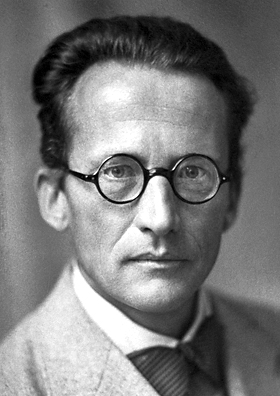
\includegraphics[width=\linewidth]{images/book4/schrodinger-1933.jpg}\par
{\footnotesize Schrödinger en 1933.}
\end{minipage}
\end{history}

\section{Exercices}

\begin{exercise}[$\star$]\label{exo:b3:quantum-model-systems:1}
Un électron est confiné dans une boîte de longueur (a) \qty{1.00}{nm}, (b)
\qty{0.50}{nm}. Calculer $E_1$ en joules et en électronvolts, ainsi que la
longueur d'onde de la transition $n = 1 \to 2$.
\end{exercise}

\begin{exercise}[$\star$]\label{exo:b3:quantum-model-systems:2}
Donner les cinq niveaux les plus bas d'une \omterm{def:b3:quantum-model-systems:box}{particule dans une boîte}
cubique, en unités de $h^2/8mL^2$, avec leurs \omterm{def:b3:quantum-model-systems:degenerate}{dégénérescences}.
\end{exercise}

\begin{exercise}[$\star$]\label{exo:b3:quantum-model-systems:3}
Calculer les \omterm{def:b3:quantum-model-systems:commutator}{commutateurs} $[\hat x^2,\hat p]$ et $[\hat p^2,\hat x]$ en les
faisant agir sur une fonction $f(x)$.
\end{exercise}

\begin{exercise}[$\star$]\label{exo:b3:quantum-model-systems:4}
% ledger: diat:HCl.Be
Avec $B = \qty{10.593}{cm^{-1}}$ pour \ce{H^{35}Cl}, donner les énergies
(en \unit{cm^{-1}}) et les \omterm{def:b3:quantum-model-systems:degenerate}{dégénérescences} des niveaux $J = 0$ à 3, ainsi
que le moment d'inertie de la molécule.
\end{exercise}

\begin{exercise}[$\star\star$]\label{exo:b3:quantum-model-systems:5}
Pour l'état $\psi_n$ d'une \omterm{def:b3:quantum-model-systems:box}{particule dans une boîte}, calculer $\langle x\rangle$ et
$\langle x^2\rangle$. Évaluer $\langle x^2\rangle$ pour $n = 1$ et le
comparer à la valeur classique $L^2/3$ d'une particule qui aurait la même
probabilité de se trouver n'importe où.
\end{exercise}

\begin{exercise}[$\star\star$]\label{exo:b3:quantum-model-systems:6}
% ledger: diat:H2.we, diat:D2.we
Calculer les \omterm{def:b3:quantum-model-systems:oscillator}{énergies de point zéro} harmoniques de \ce{H2} et de \ce{D2}
en \unit{kJ/mol} à partir de $\tilde\omega_e = \qty{4401.2}{cm^{-1}}$ et
\qty{3115.5}{cm^{-1}}, ainsi que leur différence. Quel rapport des nombres
d'onde attend-on d'après les \omterm{def:b3:quantum-model-systems:oscillator}{masses réduites}, et de combien le rapport
mesuré s'en approche-t-il~?
\end{exercise}

\begin{exercise}[$\star\star$]\label{exo:b3:quantum-model-systems:7}
La fonction $\phi = Nx(L - x)$ est une estimation grossière de l'état
fondamental de la boîte. La normer, puis calculer son recouvrement
$\langle\psi_1|\phi\rangle$ avec le véritable état fondamental.
\end{exercise}

\begin{exercise}[$\star\star$]\label{exo:b3:quantum-model-systems:8}
Montrer que $\hat p = -\iu\hbar\,\dd/\dd x$ est \omterm{def:b3:quantum-model-systems:hermitian}{hermitien} pour des
fonctions qui s'annulent aux extrémités d'un intervalle, et que
$\hat x\hat p$ ne l'est pas.
\end{exercise}

\begin{exercise}[$\star\star$]\label{exo:b3:quantum-model-systems:9}
Modéliser l'hexa-1,3,5-triène par six électrons $\pi$ dans une boîte de longueur $6l$, $l =
\qty{139.7}{pm}$ (cinq liaisons et une demi-liaison à chaque extrémité).
Prévoir la longueur d'onde de sa première absorption. La molécule
est-elle colorée~?
\end{exercise}

\begin{exercise}[$\star\star\star$]\label{exo:b3:quantum-model-systems:10}
Pour la barrière modèle de la figure ($V_0 = \qty{0.40}{eV}$, $a = \qty{50}{pm}$)
à $E = V_0/2$, calculer $\kappa$ pour un proton et pour un deutéron et, à
l'aide de la formule de la barrière épaisse, le rapport $T_H/T_D$. Le
comparer au rapport exact, 58.
\end{exercise}

\begin{exercise}[$\star\star\star$]\label{exo:b3:quantum-model-systems:11}
Traiter les six électrons $\pi$ du benzène comme des particules sur un
cercle de rayon \qty{139.7}{pm} (la distance C--C est égale au rayon d'un
hexagone régulier). Remplir les niveaux, puis calculer la longueur d'onde
de la transition du plus haut niveau occupé vers le plus bas niveau
vacant.
\end{exercise}

\begin{exercise}[$\star\star\star$]\label{exo:b3:quantum-model-systems:12}
Pour l'état $1s$ de l'hydrogène, $\psi = (\pi a^3)^{-1/2}\eu^{-r/a}$.
Calculer les \omterm{def:b3:quantum-model-systems:hermitian}{valeurs moyennes} $\langle r\rangle$ et $\langle V\rangle$, et
vérifier que
$\langle V\rangle = 2E_1$. (On utilisera $\int_0^\infty r^n\eu^{-\beta r}\dd r =
n!/\beta^{n+1}$.)
\end{exercise}

\section{Problème~: quelle est la longueur d'un colorant~?}

\begin{problem}[{Problème du week-end --- le modèle de l'électron libre
appliqué à trois colorants cyanines~: pourquoi une chaîne nue échoue,
quelles transitions sont permises, les échelles d'énergie d'une
molécule, et la longueur de boîte qui convient}]
\label{pb:b3:quantum-model-systems:1}
% ledger: uvvis:cyanine, uvvis:carbocyanine, uvvis:dicarbocyanine, geo:C6H6.rCC, diat:HCl.we, diat:HCl.Be
Trois colorants cyanines symétriques absorbent à 524, 603 et 711 nm dans
l'éthanol~; leurs chaînes conjuguées, entre les deux azotes et en les
incluant, comptent $j = 5$, 7
et 9 atomes. On prendra chaque liaison égale à $l = \qty{139.7}{pm}$, $m_e =
\qty{9.109e-31}{kg}$, $h = \qty{6.626e-34}{J.s}$, $c = \qty{2.998e8}{m/s}$,
$k = \qty{1.381e-23}{J/K}$, $\qty{1}{eV} = \qty{1.602e-19}{J}$.

\medskip\noindent\textbf{Partie I --- Une chaîne nue.}
\begin{enumerate}
  \item Expliquer pourquoi une chaîne de $j$ atomes porte $N = j + 1$
        électrons $\pi$, et donner $N$ pour chaque colorant.
  \item Quels niveaux de la boîte sont le plus haut occupé et le plus bas
        vacant pour le premier colorant~?
  \item Montrer que la première absorption se situe à $\lambda = 8mcL^2/h(N+1)$.
  \item Donner la longueur nue $L_0 = (j - 1)l$ de chaque chaîne.
  \item Calculer $\lambda$ pour chaque colorant avec $L = L_0$.
  \item Comparer aux valeurs mesurées. Dans quel sens le modèle se
        trompe-t-il, et qu'en déduire sur $L$~?
\end{enumerate}

\medskip\noindent\textbf{Partie II --- Quelles transitions sont permises.}
L'intensité d'une transition $n \to n'$ est proportionnelle à $|\langle
\psi_n|x - L/2|\psi_{n'}\rangle|^2$.
\begin{enumerate}[resume]
  \item Montrer que $\psi_n$ est symétrique par rapport au centre de la
        boîte pour $n$ impair et antisymétrique pour $n$ pair.
  \item En déduire que l'intégrale s'annule quand $n + n'$ est pair.
  \item La transition HOMO $\to$ LUMO de chaque colorant est-elle
        permise~?
  \item Pour le deuxième colorant, la transition de la HOMO vers le niveau
        situé au-dessus de la LUMO est-elle permise~? Celle du niveau situé
        sous la HOMO vers la LUMO~?
  \item Dans le modèle, à quelle longueur d'onde (en fraction de la
        première) se situerait la transition permise suivante depuis la
        HOMO~?
  \item Pourquoi une telle règle, tirée de la seule symétrie,
        résiste-t-elle à la grossièreté du modèle~?
\end{enumerate}

\medskip\noindent\textbf{Partie III --- Les échelles d'énergie d'une molécule.}
\begin{enumerate}[resume]
  \item Convertir l'absorption du deuxième colorant en une énergie en eV.
  \item La vibration de \ce{HCl} a $\tilde\omega_e = \qty{2991}{cm^{-1}}$~:
        convertir son quantum en eV.
  \item La rotation de \ce{HCl} a $B = \qty{10.59}{cm^{-1}}$~: convertir
        l'écart entre $J = 0$ et $J = 1$ en meV.
  \item Calculer $kT$ en meV à \qty{298}{K}.
  \item Quels types d'excitation sont peuplés à température ambiante~?
  \item Dans quels domaines du spectre observe-t-on les transitions
        électroniques, de vibration et de rotation~?
\end{enumerate}

\medskip\noindent\textbf{Partie IV --- La boîte qui convient.}
\begin{enumerate}[resume]
  \item À partir des 603 nm mesurés, calculer la longueur $L$ que doit
        avoir la boîte du deuxième colorant.
  \item En écrivant $L = L_0 + 2\delta$, en déduire $\delta$.
  \item Avec ce $\delta$, prévoir $\lambda$ pour le premier colorant~;
        donner l'écart relatif.
  \item Même question pour le troisième colorant.
  \item Interpréter $\delta$~: où vont les électrons $\pi$ au-delà des
        azotes~?
  \item Exprimer $\delta$ en longueurs de liaison, et énoncer le résultat
        du problème~: l'allongement effectif de la boîte à chaque
        extrémité.
\end{enumerate}
\end{problem}
